%\documentclass[beamer]{standalone}
%
%\begin{document}
%	\begin{frame}
%		\color{blue}\centering\Huge{\textbf{Campo Magnetico}}	
%	\end{frame}
%	
%	\begin{frame}{{Campo Magnetico}}
%		\centering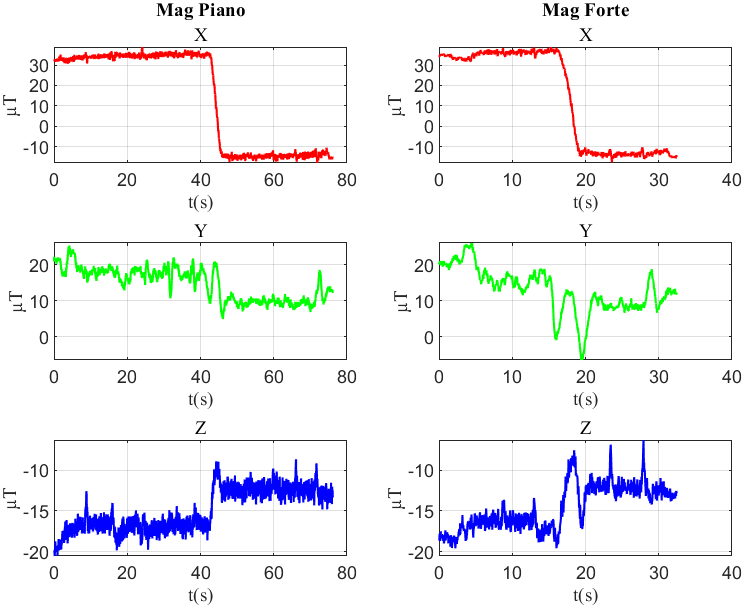
\includegraphics[height=.8\textheight]{figure/Mag/Mag}
%	\end{frame}
%	
%	\begin{frame}{{Media}}
%		\centering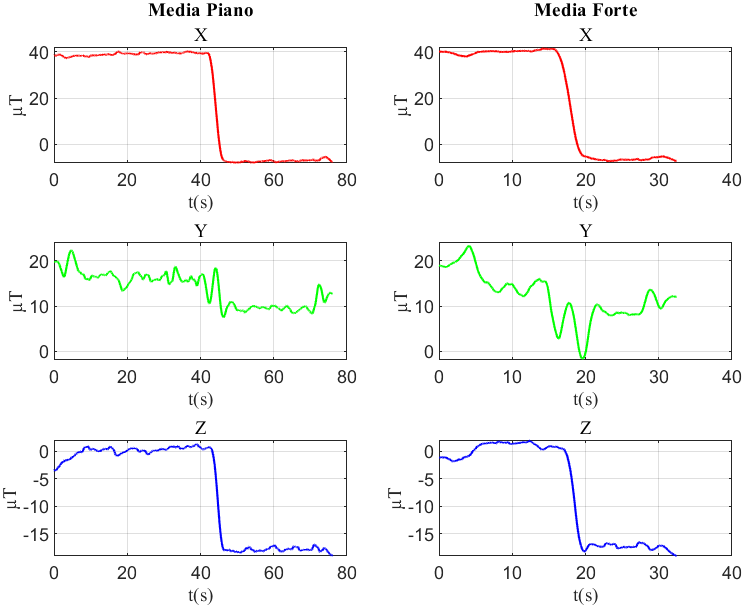
\includegraphics[height=.8\textheight]{figure/Mag/Media}
%	\end{frame}
%	
%%	\begin{frame}{{Media Rettificata}}
%%		\centering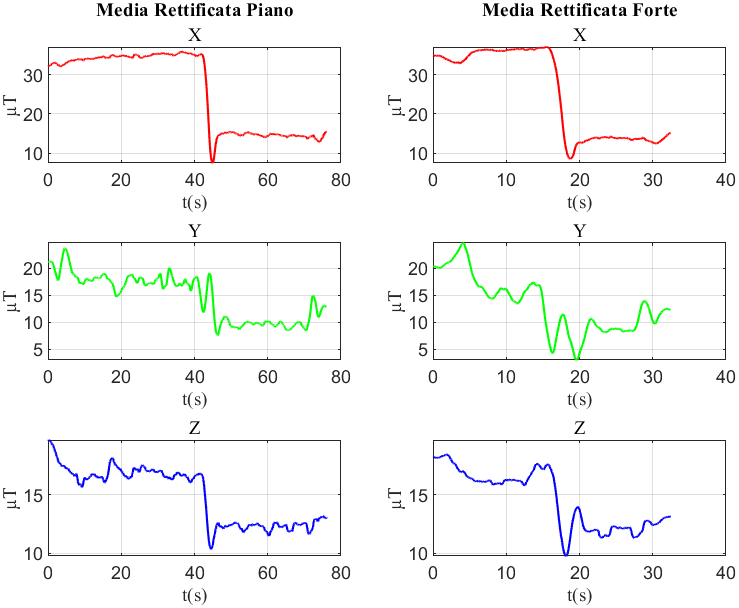
\includegraphics[height=.8\textheight]{figure/Mag/Media Rettificata}
%%	\end{frame}
%	
%	\begin{frame}{{Varianza}}
%		\centering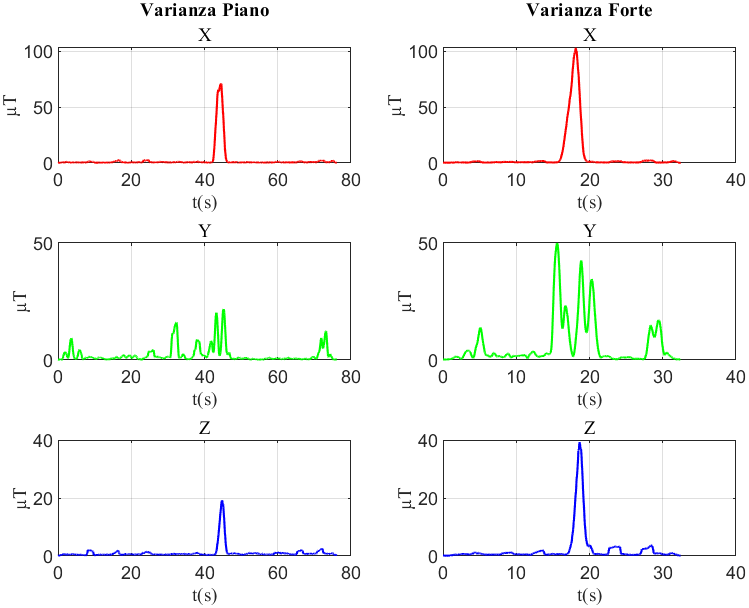
\includegraphics[height=.8\textheight]{figure/Mag/Varianza}
%	\end{frame}
%	
%%	\begin{frame}{{Deviazione Standard}}
%%		\centering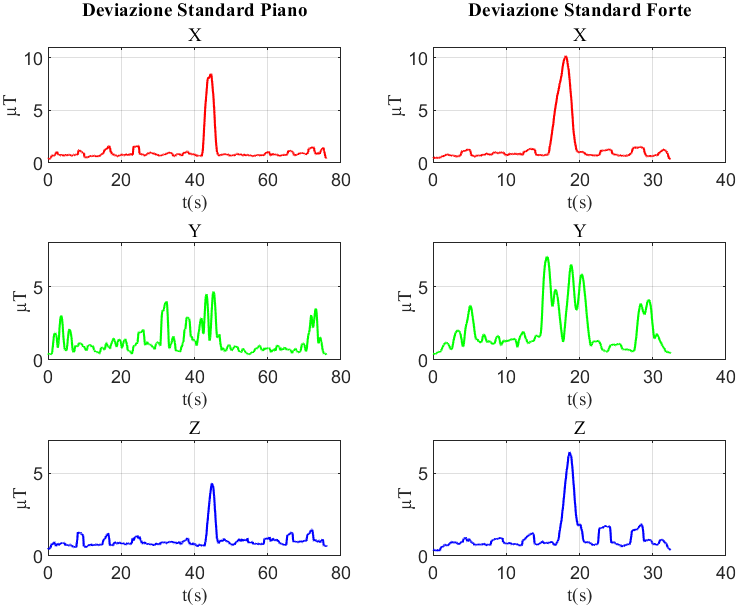
\includegraphics[height=.8\textheight]{figure/Mag/Deviazione Standard}
%%	\end{frame}
%	
%%	\begin{frame}{{Scarto Quadratico Medio}}
%%		\centering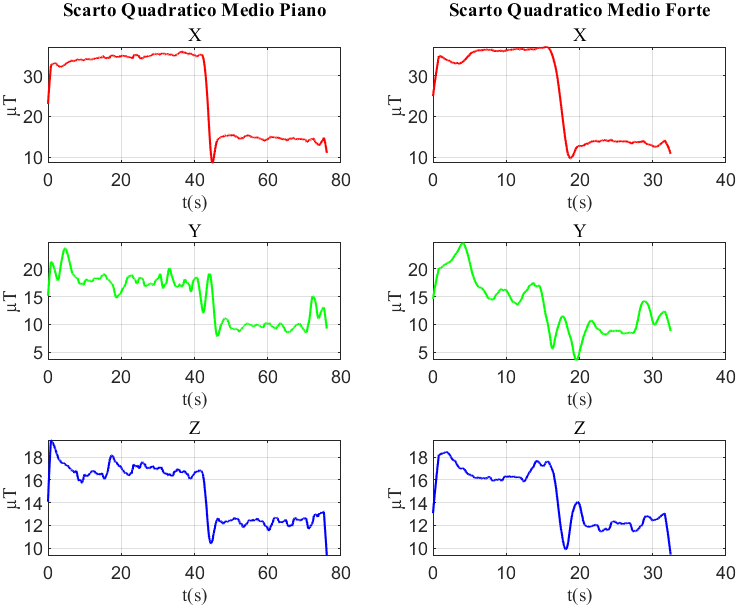
\includegraphics[height=.8\textheight]{figure/Mag/Scarto Quadratico Medio}
%%	\end{frame}
%	
%%	\begin{frame}{{Max}}
%%		\centering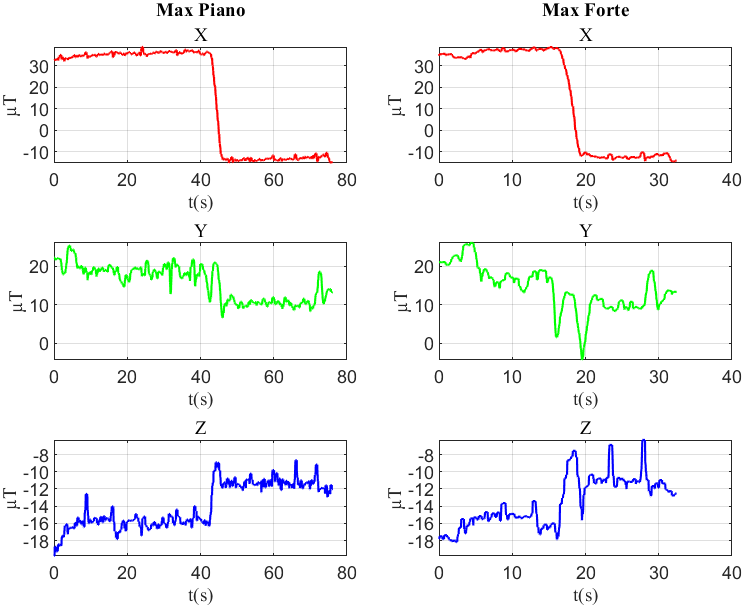
\includegraphics[height=.8\textheight]{figure/Mag/Max}
%%	\end{frame}
%%	
%%	\begin{frame}{{Min}}
%%		\centering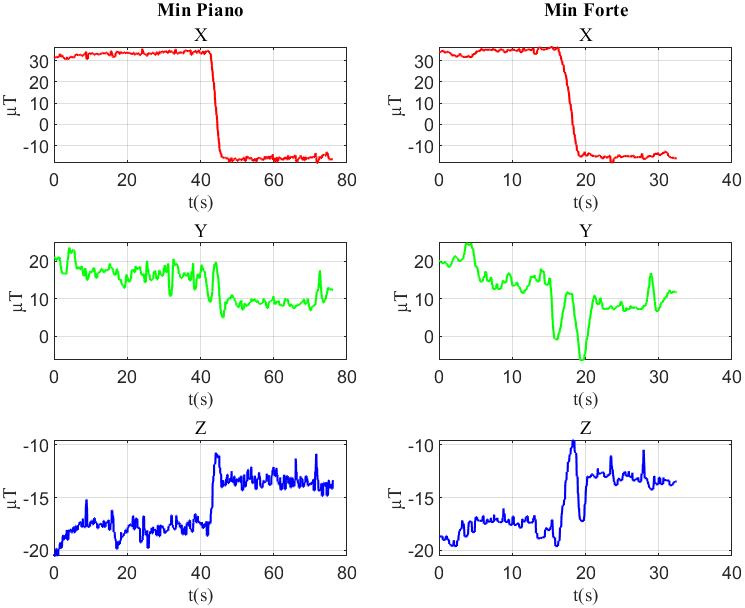
\includegraphics[height=.8\textheight]{figure/Mag/Min}
%%	\end{frame}
%%	
%%	\begin{frame}{{Peak}}
%%		\centering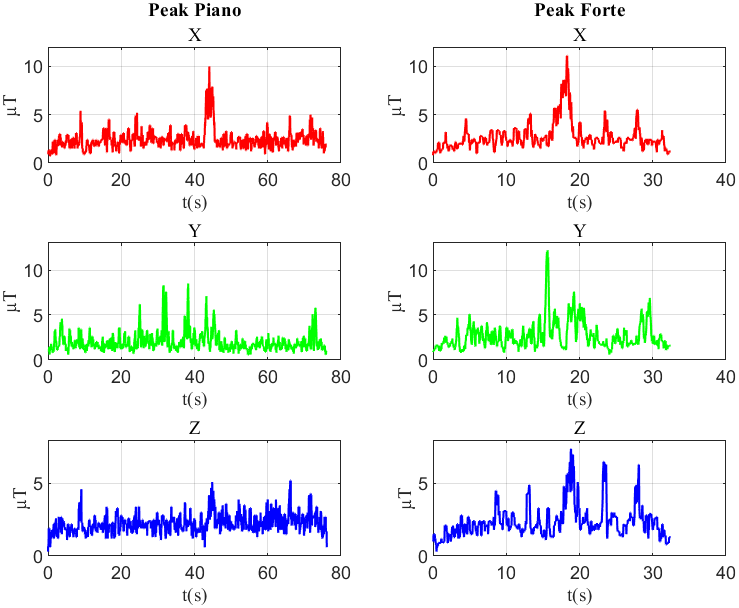
\includegraphics[height=.8\textheight]{figure/Mag/Peak}
%%	\end{frame}
%	
%%	\begin{frame}{{Kurtosi}}
%%		\centering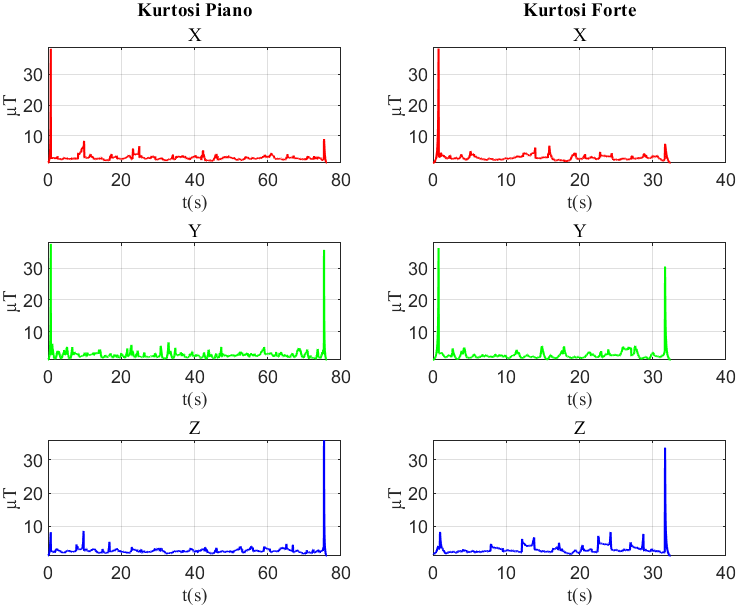
\includegraphics[height=.8\textheight]{figure/Mag/Kurtosi}
%%	\end{frame}
%%	
%%	\begin{frame}{{Skewness}}
%%		\centering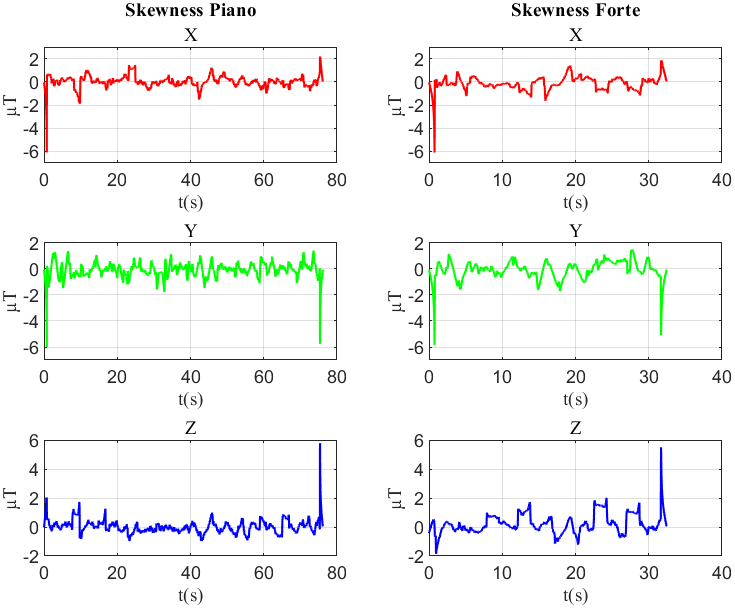
\includegraphics[height=.8\textheight]{figure/Mag/Skewness}
%%	\end{frame}
%%	
%%	\begin{frame}{{Shape Factor}}
%%		\centering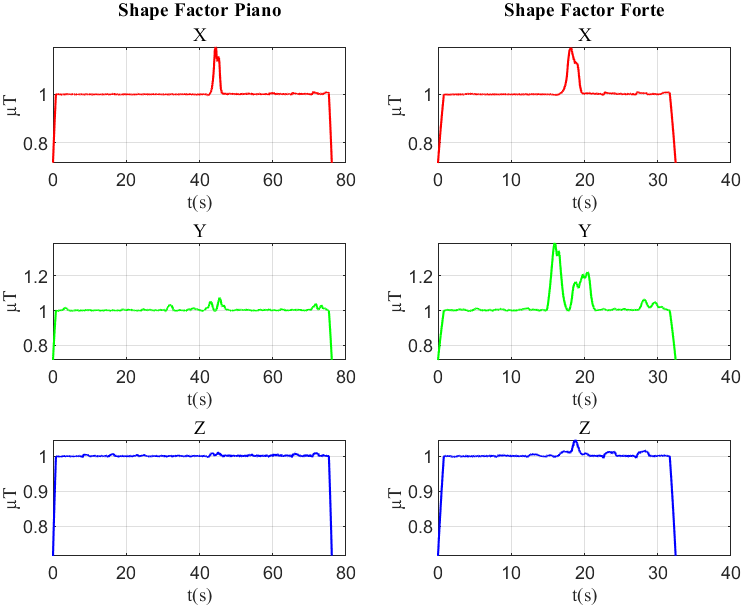
\includegraphics[height=.8\textheight]{figure/Mag/Shape Factor}
%%	\end{frame}
%%	
%%	\begin{frame}{{Crest Factor}}
%%		\centering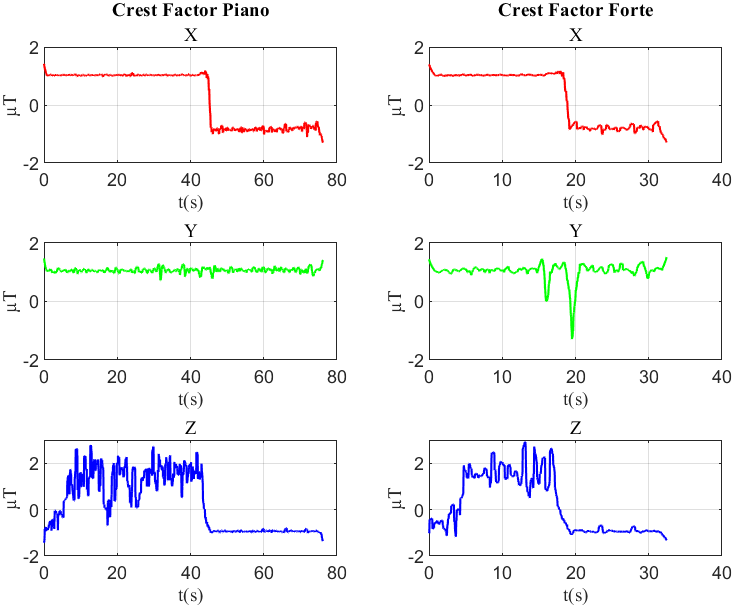
\includegraphics[height=.8\textheight]{figure/Mag/Crest Factor}
%%	\end{frame}
%%	
%%	\begin{frame}{{Impulse Factor}}
%%		\centering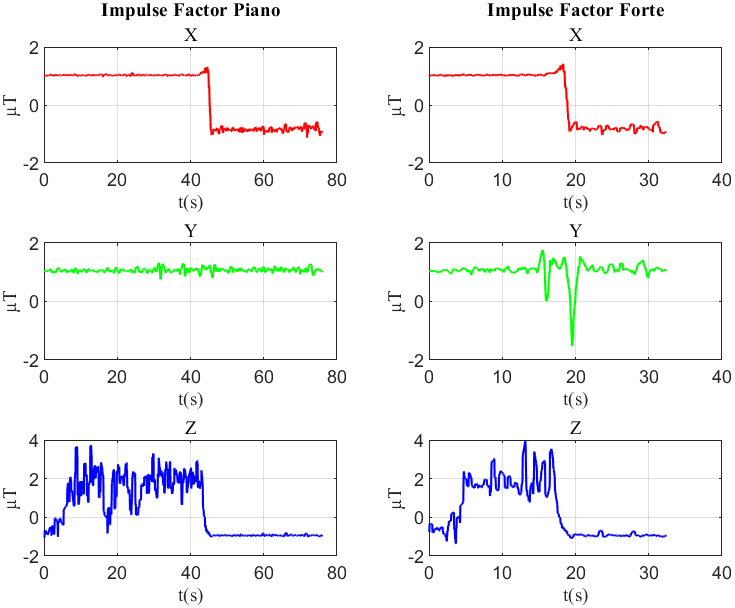
\includegraphics[height=.8\textheight]{figure/Mag/Impulse Factor}
%%	\end{frame}
%%	
%%	\begin{frame}{{Margin Factor}}
%%		\centering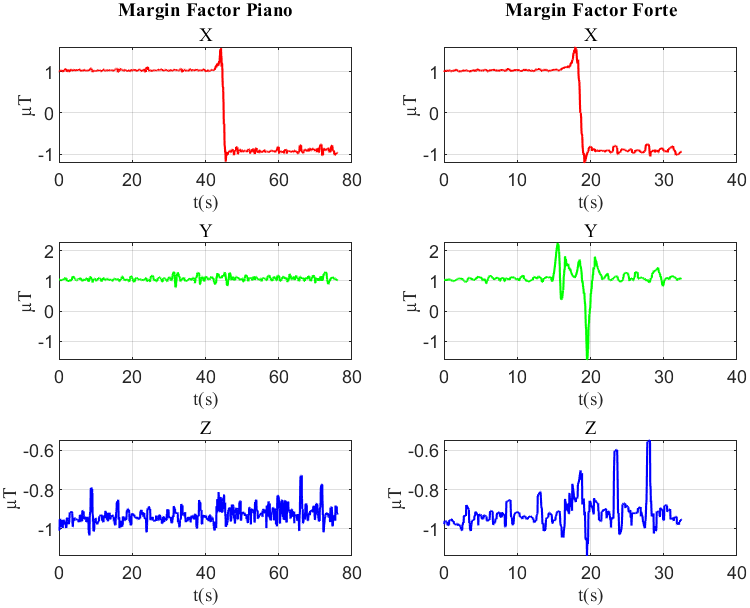
\includegraphics[height=.8\textheight]{figure/Mag/Margin Factor}
%%	\end{frame}
%	
%	\begin{frame}{{Trasformata}}
%		\centering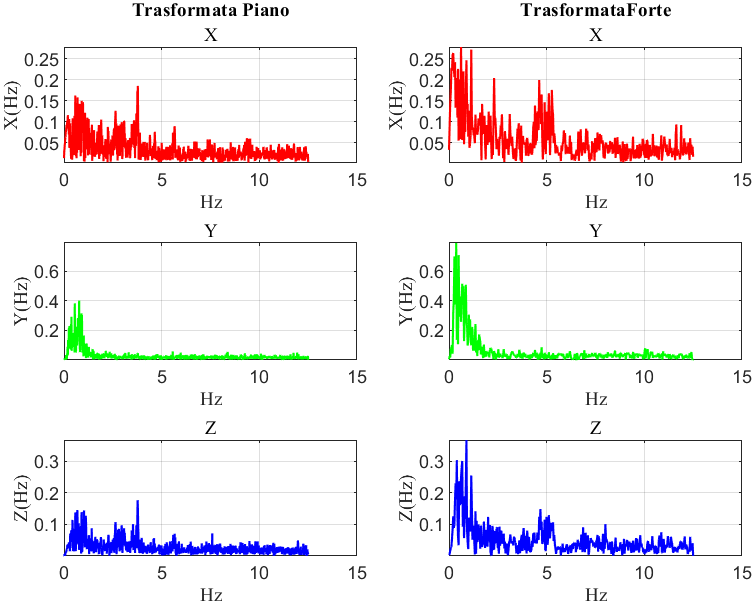
\includegraphics[height=.8\textheight]{figure/Mag/Trasformata/Trasformata}
%	\end{frame}
%	
%	\begin{frame}{{Spettro}}
%		\centering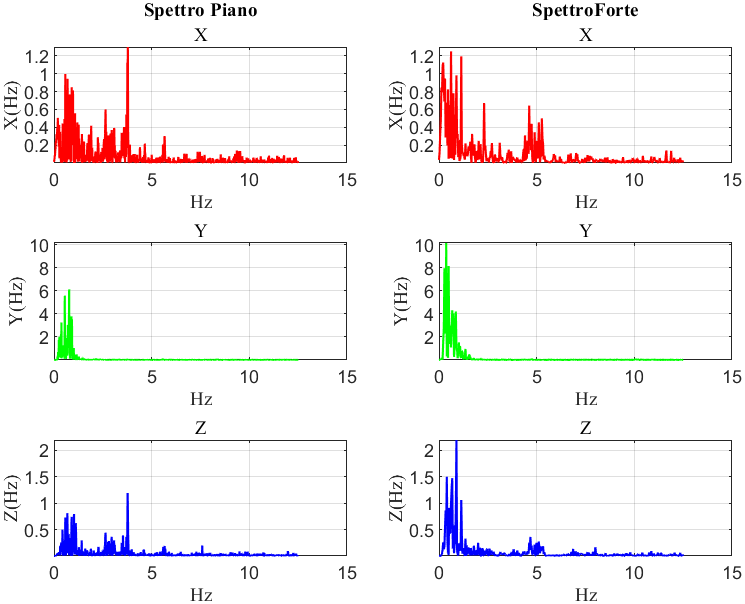
\includegraphics[height=.8\textheight]{figure/Mag/Trasformata/Spettro}
%	\end{frame}
%	
%	\begin{frame}
%		\color{blue}\centering\huge{\textbf{Trasformata Campo Magnetico}}
%	\end{frame}
%	
%	\begin{frame}{{Ampiezza Media X}}					
%		\centering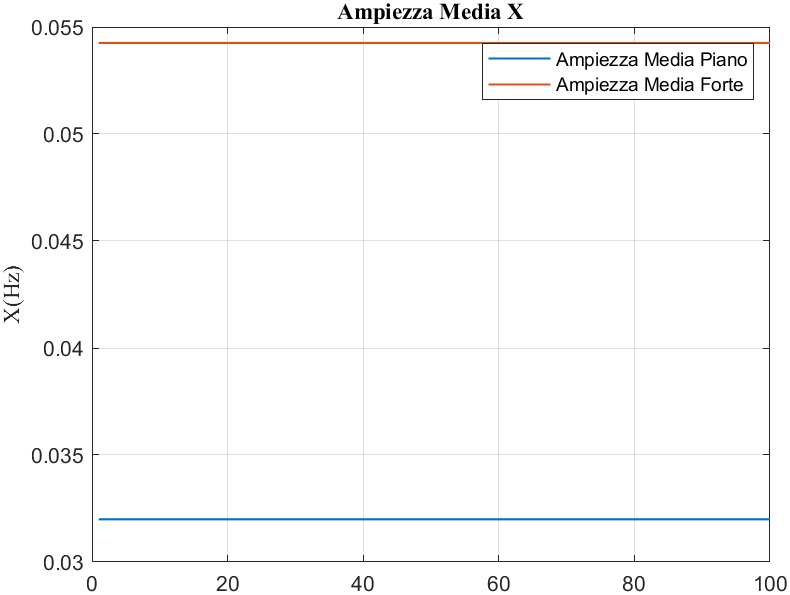
\includegraphics[height=.8\textheight]{figure/Mag/Trasformata/Ampiezza MediaX}
%	\end{frame}
%	
%	\begin{frame}{{Ampiezza Media Y}}					
%		\centering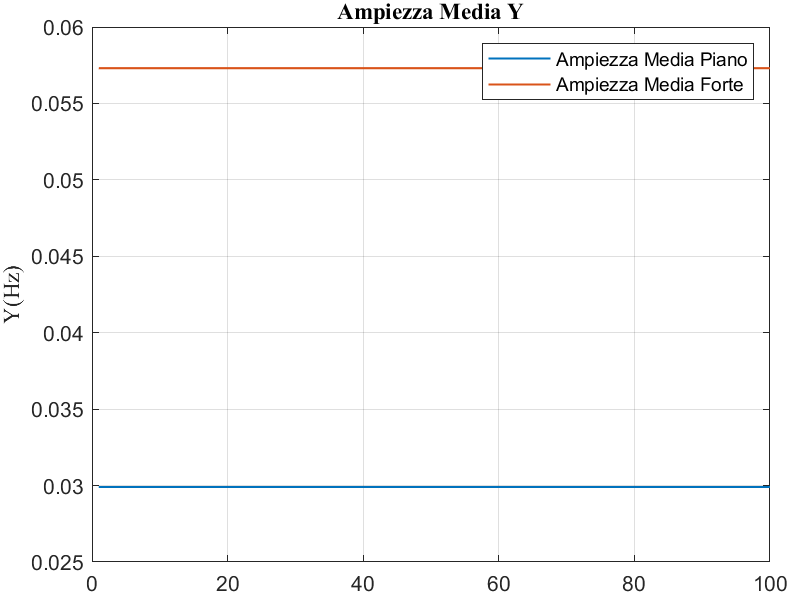
\includegraphics[height=.8\textheight]{figure/Mag/Trasformata/Ampiezza MediaY}
%	\end{frame}
%	
%	\begin{frame}{{Ampiezza Media Z}}					
%		\centering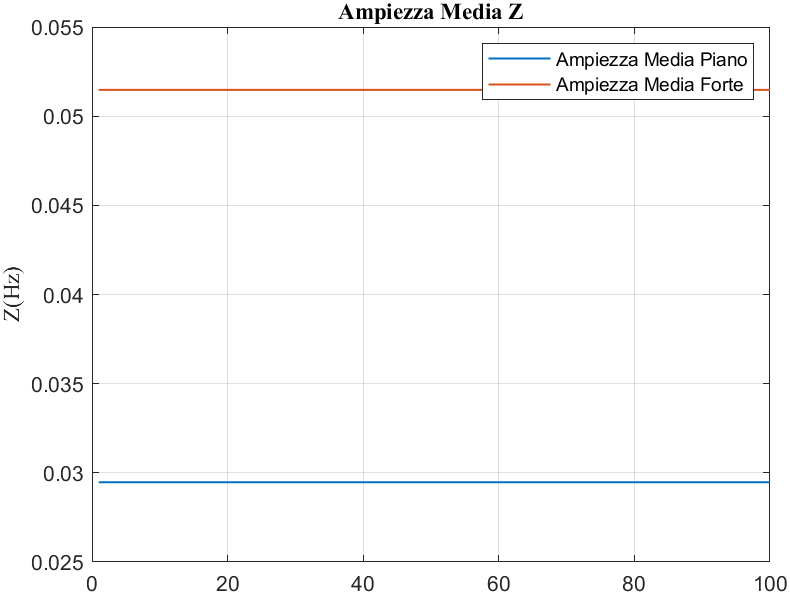
\includegraphics[height=.8\textheight]{figure/Mag/Trasformata/Ampiezza MediaZ}
%	\end{frame}
%	
%	\begin{frame}{{Frequency Centroid X}}
%		\centering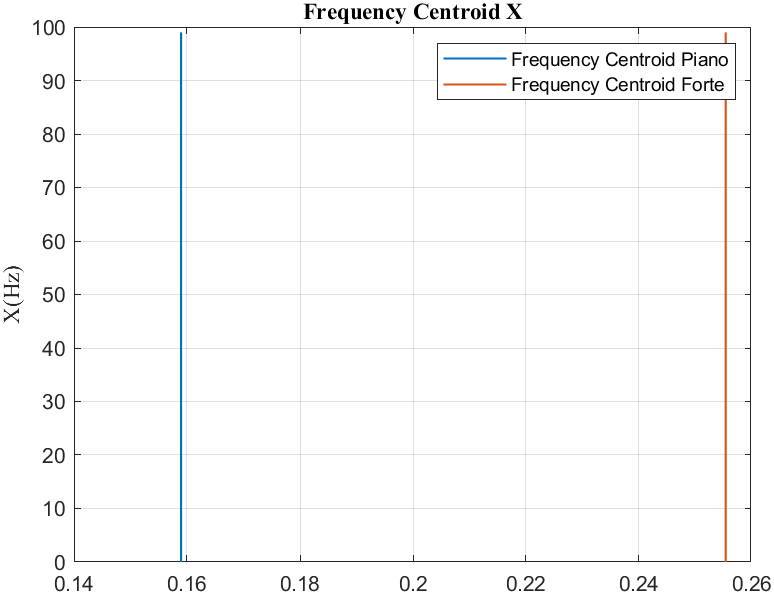
\includegraphics[height=.8\textheight]{figure/Mag/Trasformata/Frequency CentroidX}
%	\end{frame}
%	
%	\begin{frame}{{Frequency Centroid Y}}
%		\centering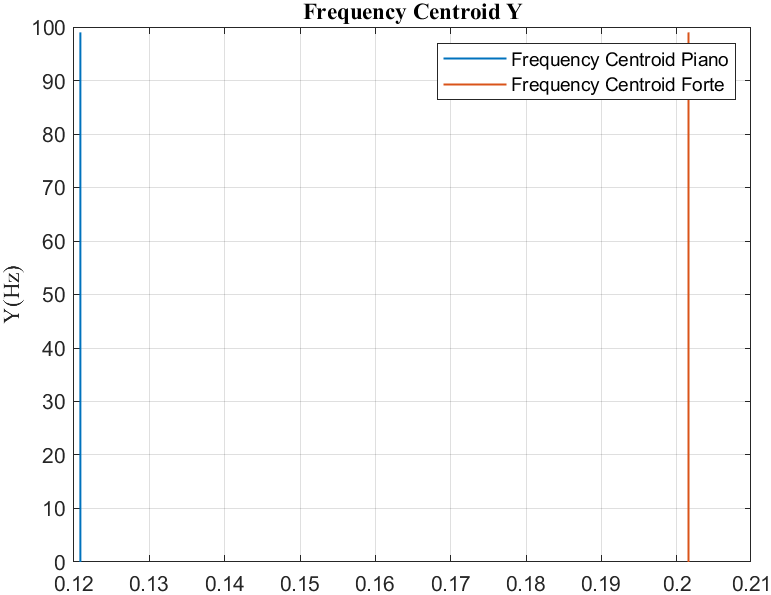
\includegraphics[height=.8\textheight]{figure/Mag/Trasformata/Frequency CentroidY}
%	\end{frame}
%	
%	\begin{frame}{{Frequency Centroid Z}}
%		\centering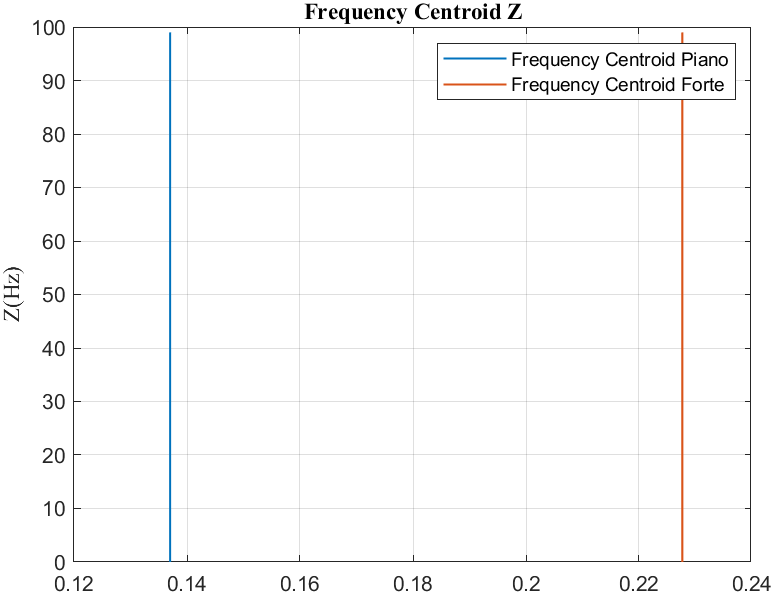
\includegraphics[height=.8\textheight]{figure/Mag/Trasformata/Frequency CentroidZ}
%	\end{frame}
%	
%	\begin{frame}{{Frequency Variance X}}
%		\centering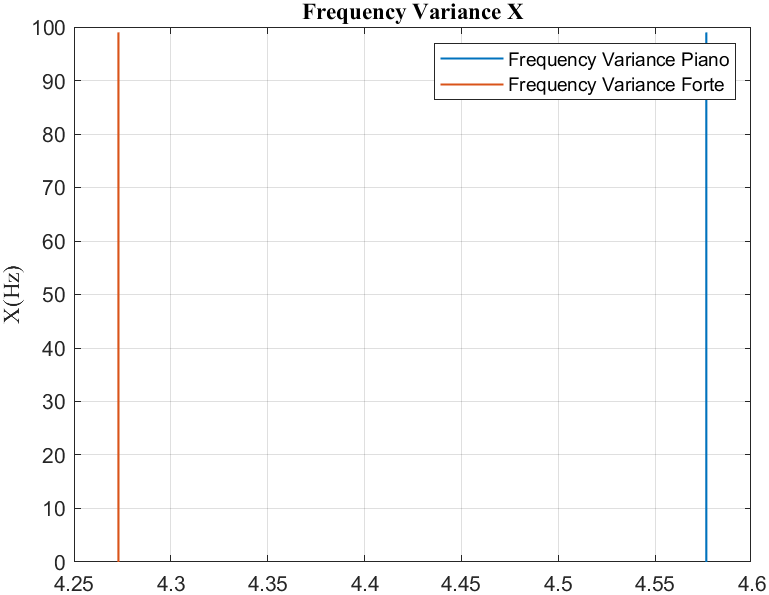
\includegraphics[height=.8\textheight]{figure/Mag/Trasformata/Frequency VarianceX}
%	\end{frame}
%	
%	\begin{frame}{{Frequency Variance Y}}
%		\centering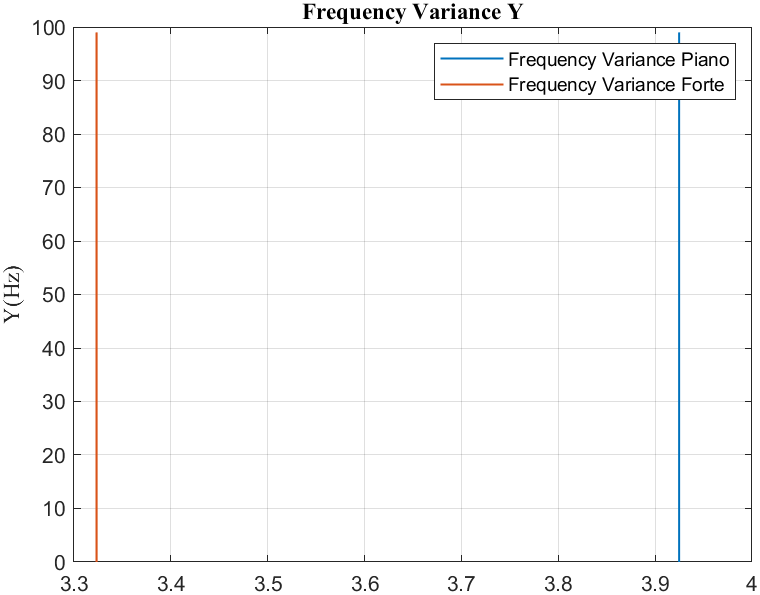
\includegraphics[height=.8\textheight]{figure/Mag/Trasformata/Frequency VarianceY}
%	\end{frame}
%	
%	\begin{frame}{{Frequency Variance Z}}
%		\centering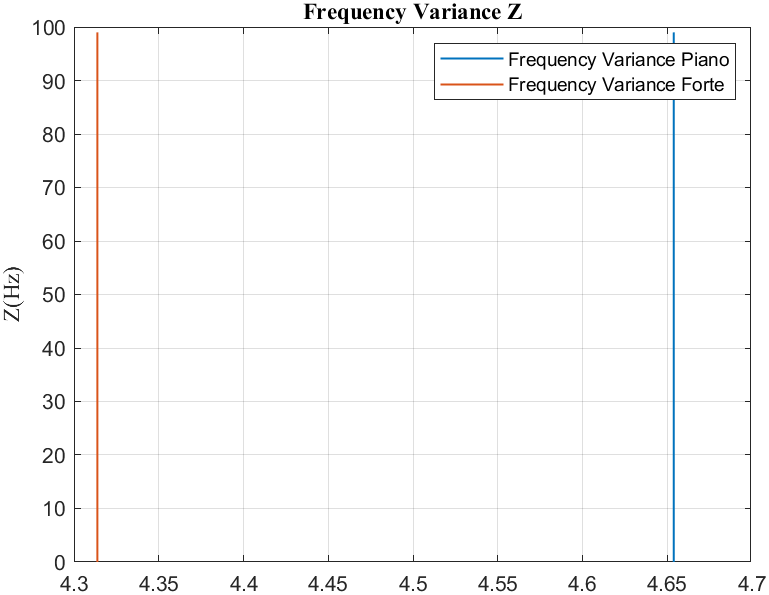
\includegraphics[height=.8\textheight]{figure/Mag/Trasformata/Frequency VarianceZ}
%	\end{frame}
%	
%	\begin{frame}
%		\color{blue}\centering\huge{\textbf{Spettro Campo Magnetico}}
%	\end{frame}
%	
%	\begin{frame}{{Spectral EntropyX}}
%		\centering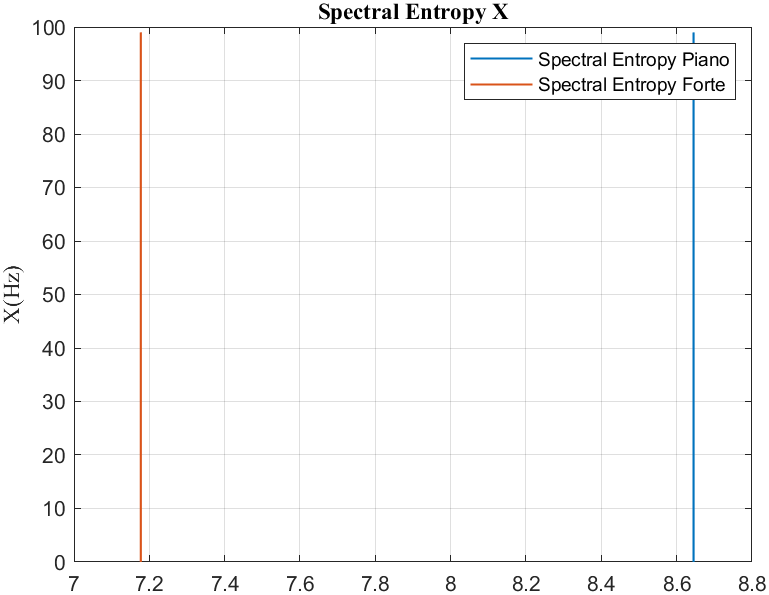
\includegraphics[height=.8\textheight]{figure/Mag/Trasformata/Spectral EntropyX}
%	\end{frame}
%	
%	\begin{frame}{{Spectral EntropyY}}
%		\centering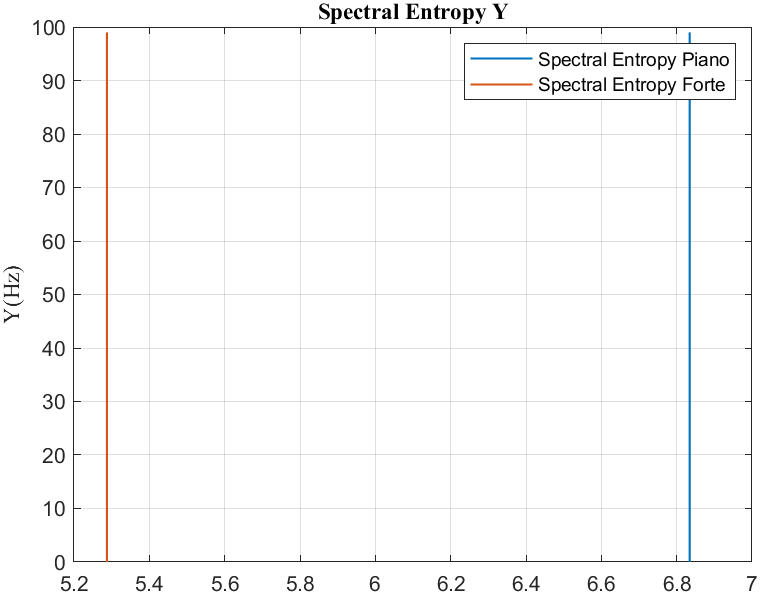
\includegraphics[height=.8\textheight]{figure/Mag/Trasformata/Spectral EntropyY}
%	\end{frame}
%	
%	\begin{frame}{{Spectral EntropyZ}}
%		\centering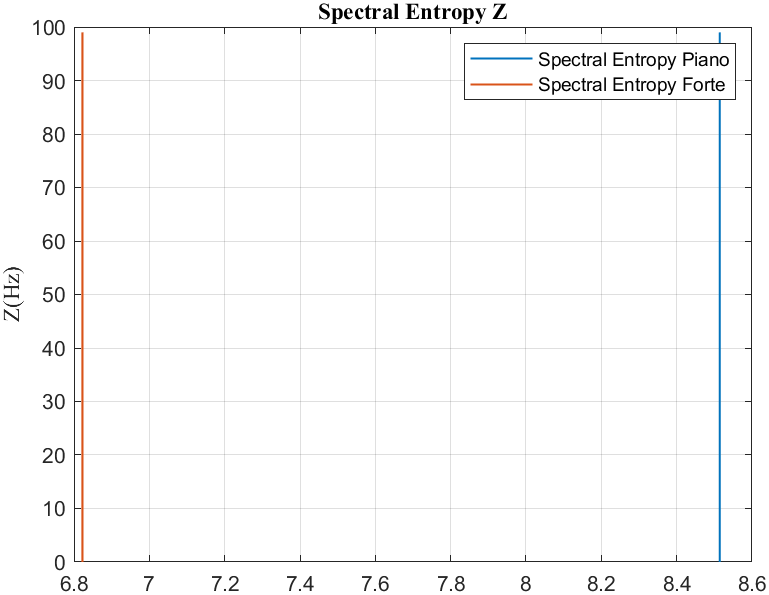
\includegraphics[height=.8\textheight]{figure/Mag/Trasformata/Spectral EntropyZ}
%	\end{frame}
%	
%\end{document}

\documentclass[beamer]{standalone}

\begin{document}
	\begin{frame}
		\color{blue}\centering\Huge{\textbf{Campo Magnetico}}	
	\end{frame}
	
	\begin{frame}{{Campo Magnetico}}
		\centering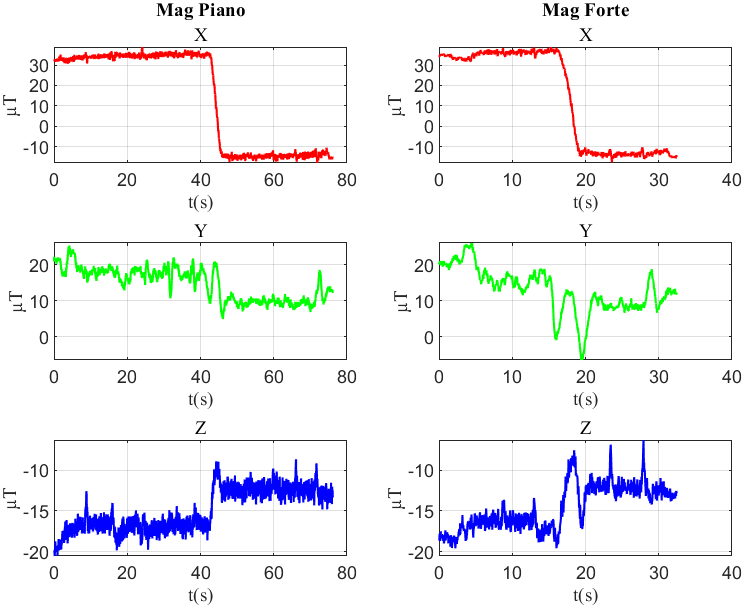
\includegraphics[height=.8\textheight]{figure/Mag/Mag}
	\end{frame}
	
	\begin{frame}{{Media}}
		\centering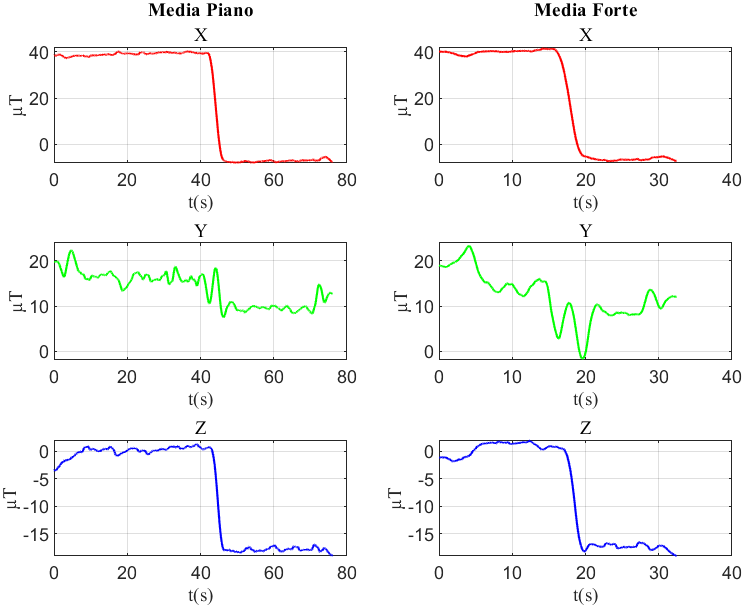
\includegraphics[height=.8\textheight]{figure/Mag/Media}
	\end{frame}
	
	\begin{frame}{{Media Rettificata}}
		\centering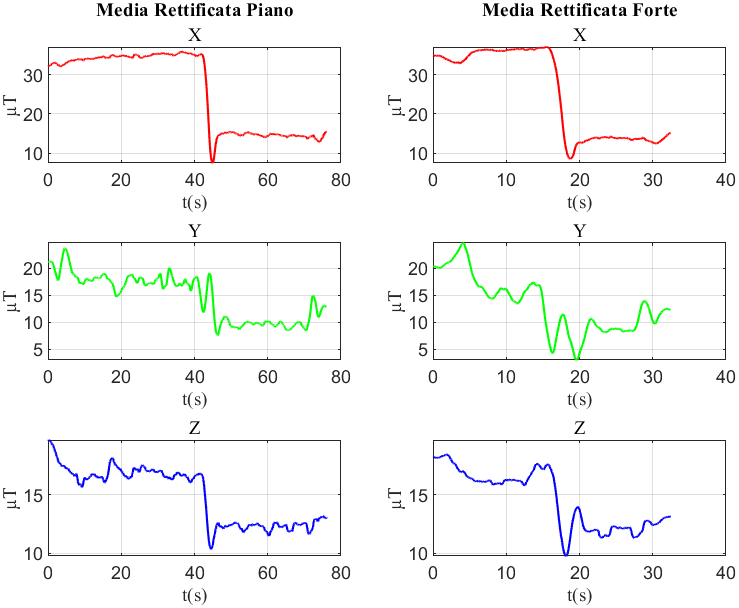
\includegraphics[height=.8\textheight]{figure/Mag/Media Rettificata}
	\end{frame}
	
	\begin{frame}{{Varianza}}
		\centering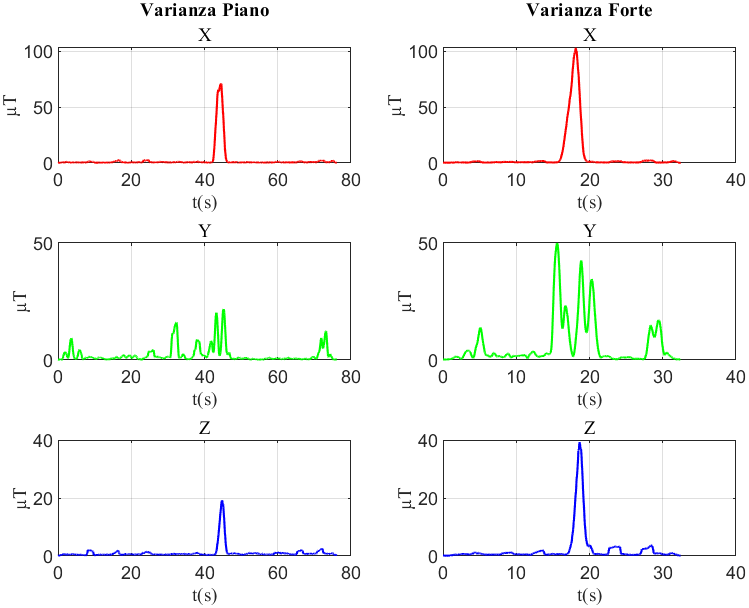
\includegraphics[height=.8\textheight]{figure/Mag/Varianza}
	\end{frame}
	
	\begin{frame}{{Deviazione Standard}}
		\centering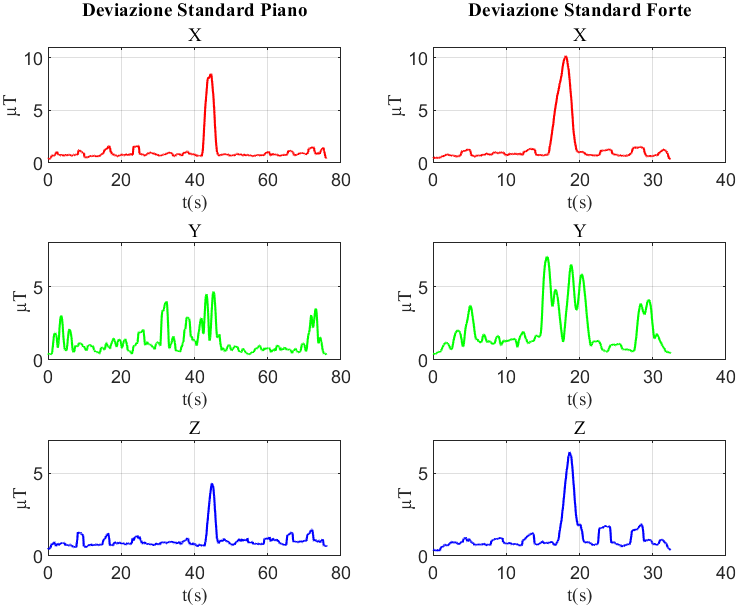
\includegraphics[height=.8\textheight]{figure/Mag/Deviazione Standard}
	\end{frame}
	
	\begin{frame}{{Scarto Quadratico Medio}}
		\centering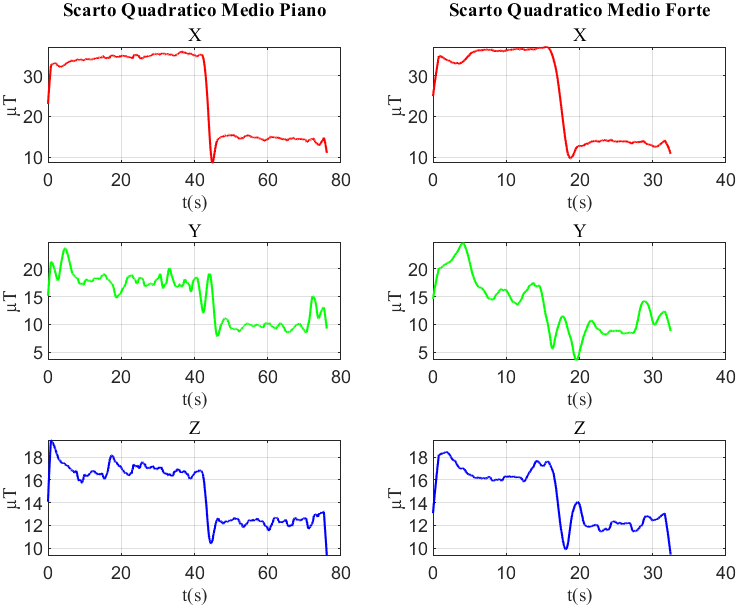
\includegraphics[height=.8\textheight]{figure/Mag/Scarto Quadratico Medio}
	\end{frame}
	
	\begin{frame}{{Max}}
		\centering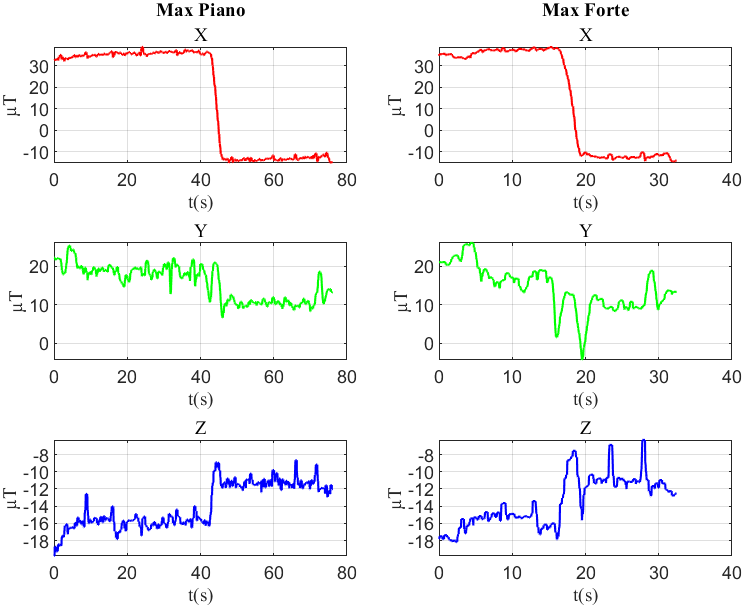
\includegraphics[height=.8\textheight]{figure/Mag/Max}
	\end{frame}
	
	\begin{frame}{{Min}}
		\centering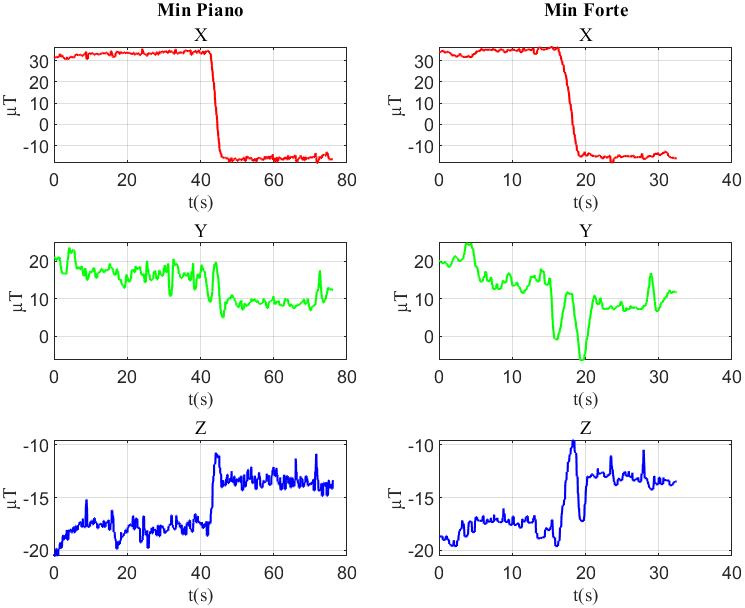
\includegraphics[height=.8\textheight]{figure/Mag/Min}
	\end{frame}
	
	\begin{frame}{{Peak}}
		\centering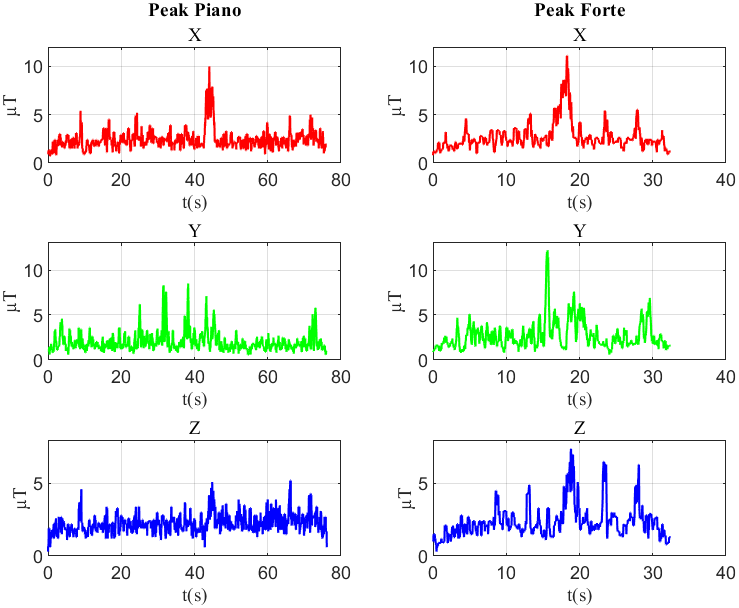
\includegraphics[height=.8\textheight]{figure/Mag/Peak}
	\end{frame}
	
	\begin{frame}{{Kurtosi}}
		\centering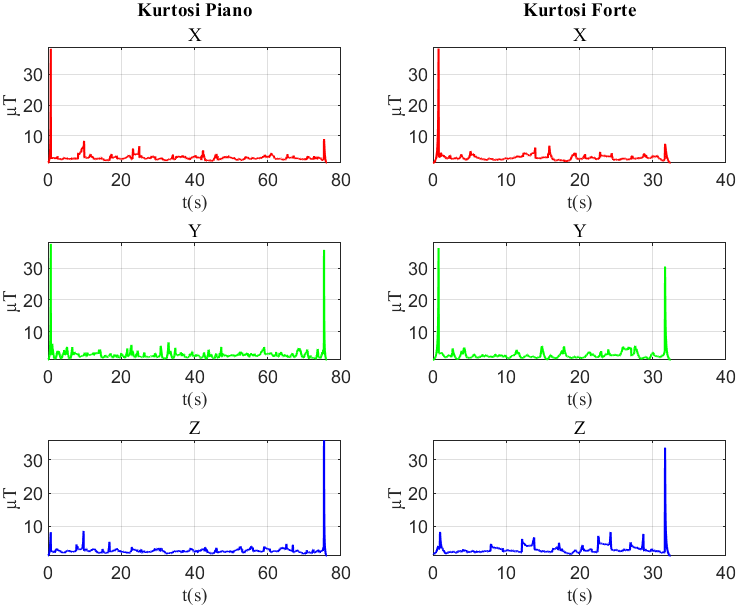
\includegraphics[height=.8\textheight]{figure/Mag/Kurtosi}
	\end{frame}
	
	\begin{frame}{{Skewness}}
		\centering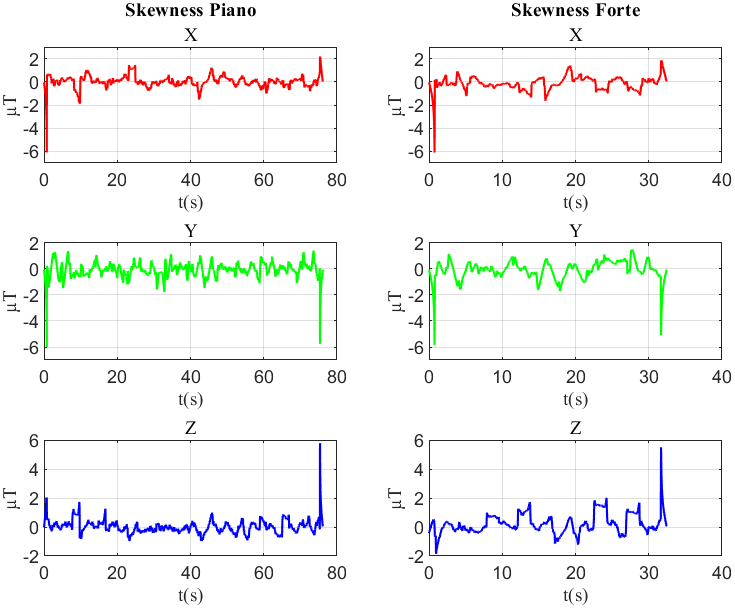
\includegraphics[height=.8\textheight]{figure/Mag/Skewness}
	\end{frame}
	
	\begin{frame}{{Shape Factor}}
		\centering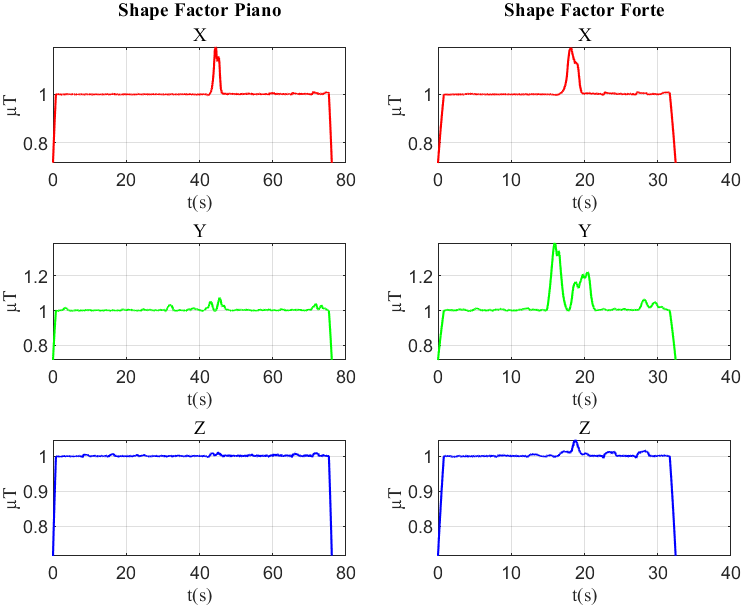
\includegraphics[height=.8\textheight]{figure/Mag/Shape Factor}
	\end{frame}
	
	\begin{frame}{{Crest Factor}}
		\centering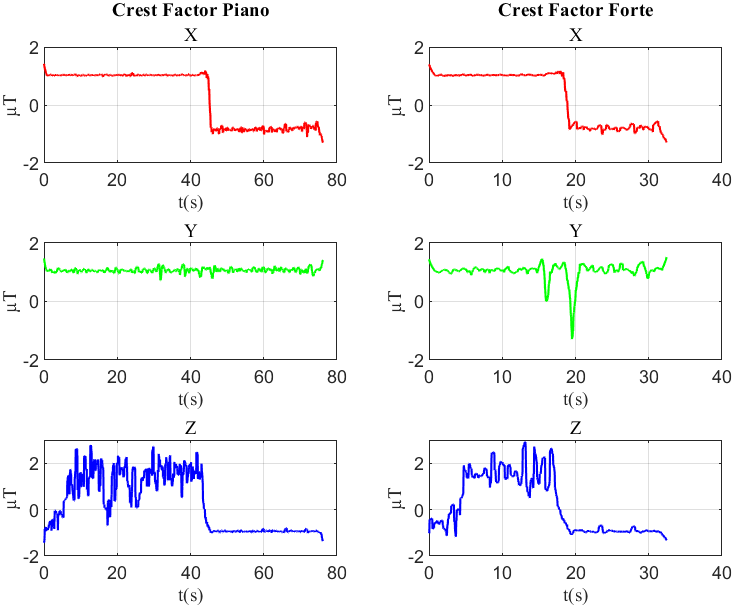
\includegraphics[height=.8\textheight]{figure/Mag/Crest Factor}
	\end{frame}
	
	\begin{frame}{{Impulse Factor}}
		\centering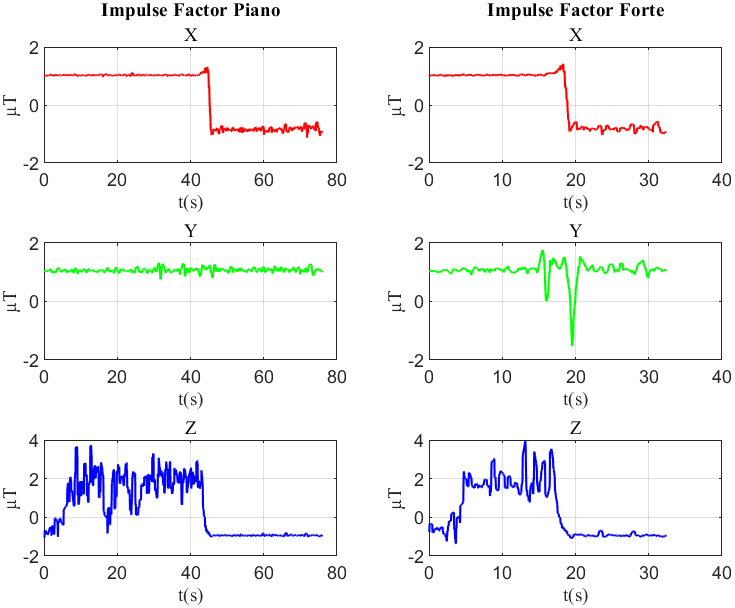
\includegraphics[height=.8\textheight]{figure/Mag/Impulse Factor}
	\end{frame}
	
	\begin{frame}{{Margin Factor}}
		\centering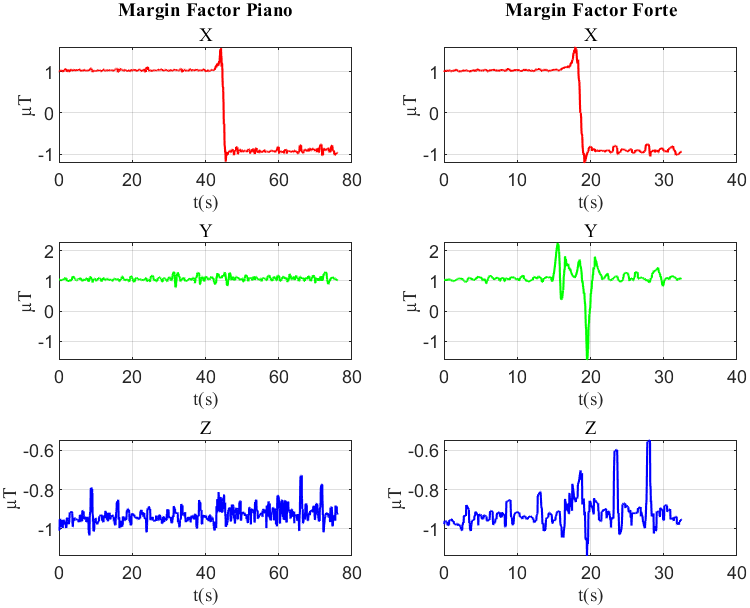
\includegraphics[height=.8\textheight]{figure/Mag/Margin Factor}
	\end{frame}
	
	\begin{frame}{{Trasformata}}
		\centering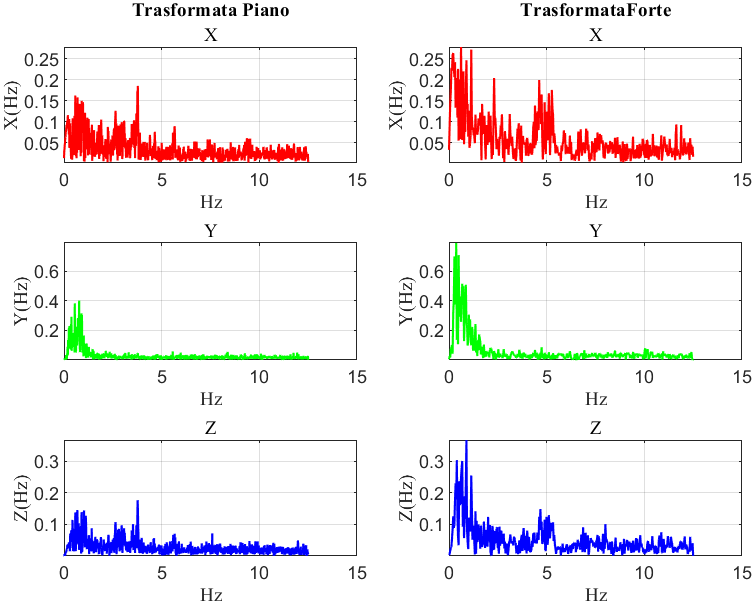
\includegraphics[height=.8\textheight]{figure/Mag/Trasformata/Trasformata}
	\end{frame}
	
	\begin{frame}{{Spettro}}
		\centering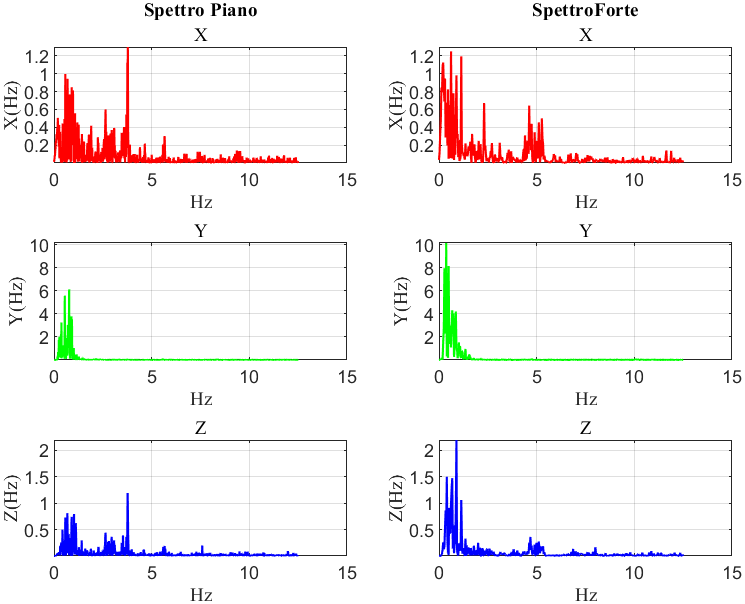
\includegraphics[height=.8\textheight]{figure/Mag/Trasformata/Spettro}
	\end{frame}
	
	\begin{frame}
		\color{blue}\centering\huge{\textbf{Trasformata Campo Magnetico}}
	\end{frame}
	
	\begin{frame}{{Ampiezza Media X}}					
		\centering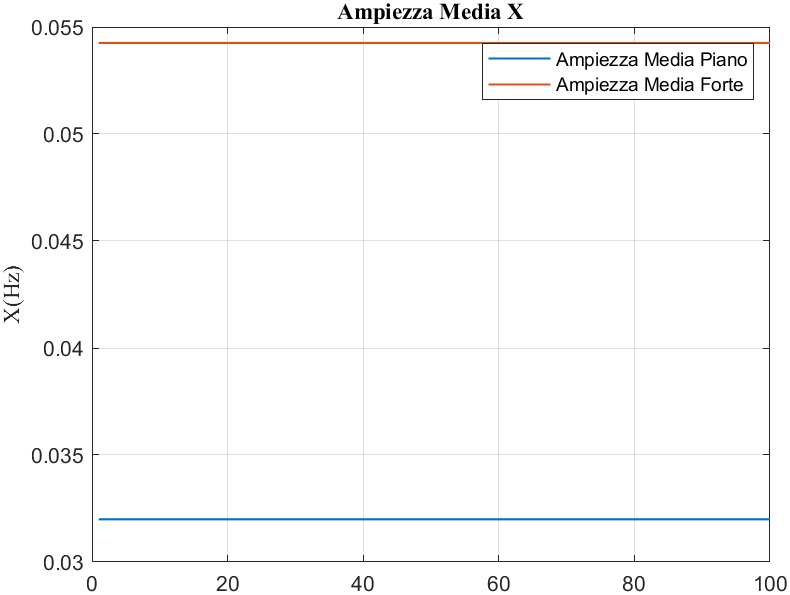
\includegraphics[height=.8\textheight]{figure/Mag/Trasformata/Ampiezza MediaX}
	\end{frame}
	
	\begin{frame}{{Ampiezza Media Y}}					
		\centering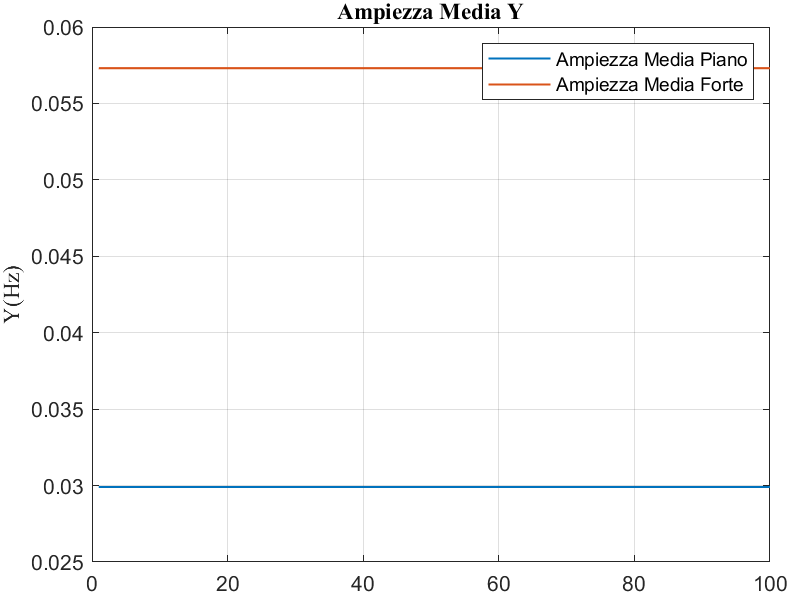
\includegraphics[height=.8\textheight]{figure/Mag/Trasformata/Ampiezza MediaY}
	\end{frame}
	
	\begin{frame}{{Ampiezza Media Z}}					
		\centering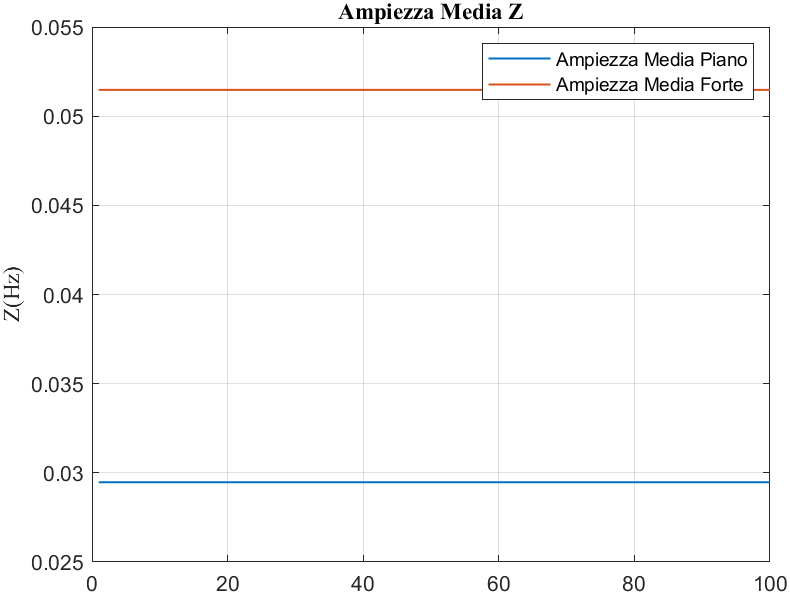
\includegraphics[height=.8\textheight]{figure/Mag/Trasformata/Ampiezza MediaZ}
	\end{frame}
	
	\begin{frame}{{Frequency Centroid X}}
		\centering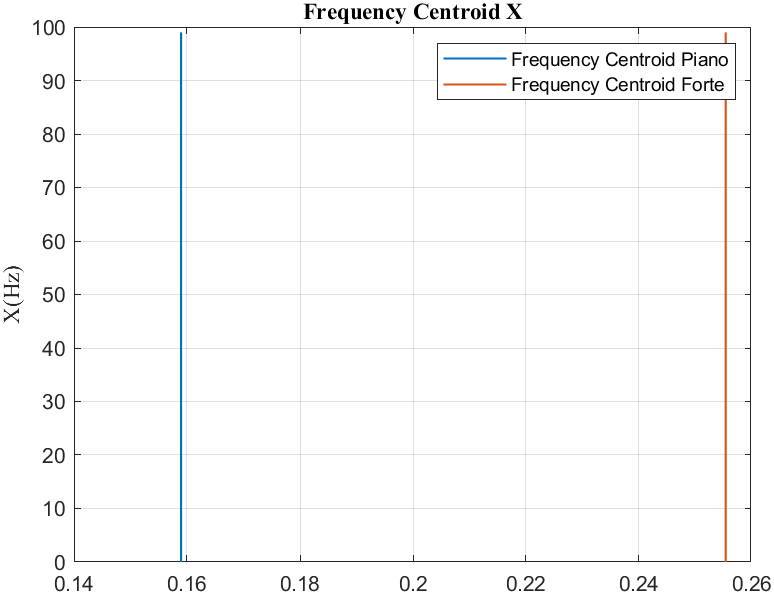
\includegraphics[height=.8\textheight]{figure/Mag/Trasformata/Frequency CentroidX}
	\end{frame}
	
	\begin{frame}{{Frequency Centroid Y}}
		\centering\includegraphics[height=.8\textheight]{figure/Mag/Trasformata/Frequency CentroidY}
	\end{frame}
	
	\begin{frame}{{Frequency Centroid Z}}
		\centering\includegraphics[height=.8\textheight]{figure/Mag/Trasformata/Frequency CentroidZ}
	\end{frame}
	
	\begin{frame}{{Frequency Variance X}}
		\centering\includegraphics[height=.8\textheight]{figure/Mag/Trasformata/Frequency VarianceX}
	\end{frame}
	
	\begin{frame}{{Frequency Variance Y}}
		\centering\includegraphics[height=.8\textheight]{figure/Mag/Trasformata/Frequency VarianceY}
	\end{frame}
	
	\begin{frame}{{Frequency Variance Z}}
		\centering\includegraphics[height=.8\textheight]{figure/Mag/Trasformata/Frequency VarianceZ}
	\end{frame}
	
	\begin{frame}
		\color{blue}\centering\huge{\textbf{Spettro Campo Magnetico}}
	\end{frame}
	
	\begin{frame}{{Spectral EntropyX}}
		\centering\includegraphics[height=.8\textheight]{figure/Mag/Trasformata/Spectral EntropyX}
	\end{frame}
	
	\begin{frame}{{Spectral EntropyY}}
		\centering\includegraphics[height=.8\textheight]{figure/Mag/Trasformata/Spectral EntropyY}
	\end{frame}
	
	\begin{frame}{{Spectral EntropyZ}}
		\centering\includegraphics[height=.8\textheight]{figure/Mag/Trasformata/Spectral EntropyZ}
	\end{frame}
	
\end{document}